\documentclass[preprint,authoryear,1p,12pt]{elsarticle}

\usepackage{lineno}
\usepackage{amsmath}
\usepackage{amssymb}
\usepackage{graphicx}
\usepackage{booktabs}
\usepackage{hyperref}
\usepackage{microtype}
\usepackage{xcolor}

\graphicspath{{../figures/}{./figures/}}

\journal{Journal of Dental Research}

\begin{document}

\begin{frontmatter}

\title{DentaCoPilot: An LLM-Augmented Next-Procedure Recommender for General Dentistry, Designed for Dentist Augmentation}

\author[celabe]{Carson Conception Rodrigues\corref{cor1}}
\ead{carson@celabe.com}
\author[kle]{Steffie Dione Rebello}

\address[celabe]{CELABE, Research Division}
\address[kle]{KLE Vishwanath Katti Institute of Dental Sciences, Belgaum, India}

\cortext[cor1]{Corresponding author.}

\begin{abstract}
\textbf{Background.} Commercial dental artificial intelligence in 2026 is overwhelmingly diagnostic: caries, calculus, periapical, and bone-level detection on radiographs. The clinically harder question that follows every diagnosis --- given a patient's chart and most recent procedure, what should the dentist do next --- remains unsolved at general-dentistry scale. The closest published system, MultiTP \citep{chen2024multitp}, is a CNN-RNN restricted to partial-edentulism cases and provides neither calibrated uncertainty, structured rationale, nor an evaluation that treats the model as decision support rather than as an autonomous classifier.
%
\textbf{Methods.} We introduce \textit{DentaCoPilot}, a recommender that, given a structured chart, returns (i) a calibrated top-$K$ probability distribution over Current Dental Terminology (CDT) codes for the next procedure, (ii) a verbalised confidence label, (iii) an explicit \textit{abstain} flag when context is insufficient, and (iv) a chart-grounded rationale. We compare four classical baselines (frequency bigram, TF-IDF + logistic regression, XGBoost, MultiTP-style CNN--RNN) and six large-language-model (LLM) variants (Claude Haiku, Sonnet + chain-of-thought, Sonnet + retrieval, Opus + chain-of-thought, Sonnet + classical prior, Opus + classical prior) on a synthetic chart corpus of 500 patients (1{,}284 test examples). All LLM inference is routed through the local Anthropic Claude Code CLI; every call is logged for full audit.
%
\textbf{Results.} On apples-to-apples evaluation, classical baselines reach 0.567 top-1 / 0.967 top-5; pure LLM variants trail at 0.267--0.467 top-1. Prompt-conditioning a Sonnet LLM on the classical baseline's top-10 candidates (M5) closes the gap: top-5 rises from 0.733 (pure Sonnet + chain-of-thought) to 0.933, matching classical baselines, while preserving rationale and abstention. Increasing the LLM backbone from Sonnet to Opus does not improve accuracy with or without priming. Calibration via temperature scaling and coverage--risk analysis is reported for the baselines.
%
\textbf{Conclusion.} Prompt-conditioning a small LLM on a classical baseline's top-K is the most cost-effective LLM design we tested for next-procedure recommendation, and the design preserves the augmentation features that distinguish the system from an autonomous classifier. A pre-registered clinician-in-the-loop evaluation at the KLE Vishwanath Katti Institute of Dental Sciences (Belgaum, India) and a real-data evaluation on the multi-institutional BigMouth dental data repository are the next stage of work.
\end{abstract}

\begin{keyword}
dental artificial intelligence \sep large language models \sep clinical decision support \sep procedure prediction \sep human-AI collaboration \sep calibrated abstention
\end{keyword}

\end{frontmatter}

\linenumbers

\section{Introduction}
\label{sec:intro}

Commercial dental AI in 2026 is overwhelmingly diagnostic. The most
recent FDA-clearance survey \citep{shujaat2026fdaai} catalogues 29
cleared products from 13 companies (Overjet, Pearl, VideaHealth, Dexis,
Perimetrics, and others) targeting single-image classification problems
--- caries detection, calculus identification, periapical radiolucency,
and periodontal bone-level measurement.\footnote{See
\cite{ada2024cdt} for the procedure code set used throughout this
paper.} Peer-reviewed evidence for clinical benefit exists for the
caries-detection variant in particular: in a cluster-randomised
cross-over trial of 22 dentists assessing bitewings,
\cite{mertens2021caries} reported that AI-assisted review raised the
mean diagnostic-accuracy area under the ROC from $0.85$ to $0.89$
($\Delta\text{AUC}{=}+0.04$, $p{<}0.05$); a follow-up trial confirmed
the gain was cost-effective at practice scale
\citep{schwendicke2022costeffectiveness}. These are valuable
deployments. They are also, individually, single-decision tools. They
do not answer the clinically harder question that follows every
diagnosis: \emph{what should the dentist do next?}

Sequencing a treatment plan from a chart is a different problem. A
two-surface posterior composite on tooth 19 leads to one set of likely
continuations; the same composite on a tooth with a prior endodontic
history leads to another; in a periodontitis patient with diabetes,
neither sequence is appropriate. The closest published system that
operates at this layer, MultiTP \citep{chen2024multitp}, is a CNN-RNN
restricted to partial-edentulism cases with a fixed five-treatment
output sequence. It does not surface calibrated uncertainty, does not
abstain when the chart context is insufficient, and was not evaluated as
a clinician-augmenting tool. The largest related effort in
periodontitis-risk prediction \citep{patel2026perio} is a risk model,
not a procedure recommender.

We propose \emph{DentaCoPilot}: an LLM-augmented next-procedure
recommender designed from the start as decision support for dentists. The
system takes a structured chart and the most recently completed procedure,
and emits four signals together: (i)~a top-$K$ probability distribution
over Current Dental Terminology codes for the next procedure;
(ii)~verbalised confidence in $\{$low, medium, high$\}$;
(iii)~an explicit \texttt{abstain} flag when the chart context is
genuinely insufficient; (iv)~a chart-grounded rationale citing specific
prior procedures and findings. The model is constrained-decoded to the
CDT 2024 vocabulary and calibrated via temperature scaling. Critically,
the contribution lies less in raw accuracy than in the framing: we
evaluate the system as a consult that augments the dentist, not as a
classifier that replaces the dentist's judgement.

We test two hypotheses on a synthetic chart corpus of 500 patients
(\S\ref{sec:data}): \textbf{(H1)} a calibrated LLM-based recommender
can match classical-baseline accuracy on next-procedure prediction
while preserving rationale and abstention; \textbf{(H2)} injecting a
classical baseline's top-$K$ candidates into the LLM prompt is the
most cost-effective LLM design for achieving (H1). We evaluate four
classical baselines, six LLM variants spanning Claude Haiku, Sonnet,
and Opus with chain-of-thought, retrieval, and prior-conditioning, and
report calibration and coverage--risk analyses. A pre-registered
clinician-in-the-loop evaluation at the KLE Vishwanath Katti Institute
of Dental Sciences (Belgaum, India) and a real-data evaluation on the
multi-institutional BigMouth dental data repository
\citep{walji2014bigmouth, walji2022bigmouth} are the planned next stage
of work.

All LLM inference in this work is routed through the local Anthropic
Claude Code CLI \citep{anthropic2026claudecode}, with full per-call
audit logs released alongside the code (see \S\ref{sec:compute}).

\section{Related Work}
\label{sec:related}

\paragraph{Diagnostic dental AI in commercial deployment.}
\cite{shujaat2026fdaai} catalogues the current FDA-cleared landscape:
caries / calculus detection (Overjet, Pearl, VideaHealth), periapical
radiolucency (Overjet, Pearl), automated dental charting (Overjet),
millimetre-precision bone-level quantification (Overjet, Pearl), 3D
cone-beam CT segmentation (Pearl), and acoustic fracture detection
(Perimetrics). These systems share a common shape: an image goes in, a
finding comes out. None plans treatment.

\paragraph{Procedure sequencing.} MultiTP
\citep{chen2024multitp} is the closest published system to what we
propose: a CNN-RNN with attention that predicts up to five sequential
treatments for partial-edentulism cases, achieving an AUC of 0.91 over
five plans. It is an EDR-only model with no calibration, no
abstention, and no clinician-augmentation evaluation. We reimplement a
minimal MultiTP-style architecture as our B3 comparator. In a related
specialty domain, \cite{li2025orthognathic} use multi-task
reinforcement learning with explainable AI to plan
orthodontic-orthognathic treatment, but the task is sufficiently different
(continuous decision-making over a longer planning horizon, narrow
specialty) that the contributions do not transfer directly to general
dentistry.

\paragraph{Risk prediction in dentistry.} \cite{patel2026perio} model
periodontitis risk on 20{,}946 adult patients with linked EHR-EDR data,
demonstrating that procedure-level structured data can support clinical
prediction; the same group has also shown that adding social
determinants of health to such models meaningfully changes risk
calibration \citep{patel2025sdoh}. \cite{varghese2025cariogram} pair
Cariogram-based caries-risk profiling with parent-oriented educational
mobile messages in a randomised trial, an example of coupling
structured risk modelling with a patient-facing digital intervention.
All three are risk models, not procedure recommenders; we position
our work as the procedure-recommendation analogue.

\paragraph{LLMs in dentistry.}
\cite{farhadinia2024llm} surveys early LLM applications in dental
practice, focusing on documentation, summarisation, and patient-facing
chat. The review explicitly flags that LLMs ``present clean, fluent
statements without communicating uncertainty,'' which is the failure mode
this paper directly addresses through calibration and abstention.
Broader medicine-LLM work \citep{singhal2023large,nori2023capabilities}
shows that capable models reach physician-level accuracy on knowledge
benchmarks, but \cite{omiye2024large} demonstrates that the same models
can propagate dangerous race-based clinical claims --- which motivates
our hard requirement for chart-grounded rationale and explicit
abstention. \cite{schwendicke2020artificial} surveys the chances and
challenges of dental AI broadly. To our knowledge, no prior work has
built and evaluated an LLM as a treatment-sequence recommender, and no
prior work has done so under a clinician-augmentation rather than
autonomy framing.

\paragraph{Calibration and abstention in clinical AI.}
Our calibration approach follows \cite{guo2017calibration} (temperature
scaling) with \cite{platt2000probabilistic} as the precursor. Coverage--
risk and selective prediction are standard tools in safety-critical ML;
we apply them to the procedure-recommendation setting and pre-register
the threshold-selection rule before any test-split unblinding.

\paragraph{Datasets.} BigMouth \citep{walji2014bigmouth,
walji2022bigmouth} is a multi-institutional dental EHR repository with
6M+ patients across multiple dental schools, accessed under a project-
review-committee proposal. Open imaging datasets relevant for chart-
context grounding include DENTEX \citep{dentex2023}, MMDental
\citep{mmdental2025}, and DenPAR \citep{denpar2025}.


\section{Methods}
\label{sec:method}

\subsection{Task formulation}
\label{sec:task}

We formulate next-procedure prediction as a single-step classification
over the Current Dental Terminology code set
\citep{ada2024cdt,kalenderian2018cdt}. A patient chart is a tuple
\(C = (D, M, H)\) where \(D\) holds demographics (age band, sex), \(M\)
is a list of medical-history flags, and \(H = (e_1, e_2, \dots, e_T)\)
is a time-ordered sequence of procedure events. Each event
\(e_t = (\tau_t, c_t, k_t)\) carries a date \(\tau_t\), a CDT code
\(c_t \in \mathcal{V}\), and an optional Universal-numbered tooth
identifier \(k_t \in \{1, \dots, 32\} \cup \{\bot\}\) following standard
ADA conventions \citep{wadia2017tooth}.

Given a chart truncated at index \(t\) (i.e.\ the dentist has just
performed \(e_t\)), the model outputs:

\begin{enumerate}
    \item A top-\(K\) probability distribution
      \(\hat{p}(c_{t+1} \mid C_{1:t}) \in \Delta^{|\mathcal{V}|}\) over
      the next procedure code, returned as the top-\(K\) codes ranked by
      probability.
    \item A confidence label \(\hat{q} \in \{\text{low, medium, high}\}\),
      a verbalised self-rating
      \citep{lin2022teaching,kadavath2022know,xiong2024can}.
    \item An abstain flag \(a \in \{0, 1\}\) which the system sets to
      \(1\) when the chart context is judged insufficient.
    \item A short rationale \(r\) grounded in cited fields of the chart
      \(C_{1:t}\) (used for evaluation, not for the prediction itself).
\end{enumerate}

We expand each chart of length \(L\) into \(L-1\) prediction examples by
truncating at every prefix index \(t \in \{1, \dots, L-1\}\). Train, dev,
and test splits are constructed at the \emph{patient} level (no chart
appears in two splits), following standard EHR-modeling practice
\citep{rajkomar2018scalable,park2024review}.

We report \textbf{top-$K$ accuracy}: the fraction of test examples for
which the gold next-procedure code appears among the model's $K$
highest-probability predictions. Top-1 corresponds to exact CDT match;
top-3 and top-5 capture clinically reasonable shortlists for a
recommender (a dentist seeing a small candidate list with calibrated
probabilities is the deployment mode we have in mind). We also report
top-1 by CDT category and, where calibrated probabilities are available,
Expected Calibration Error and coverage--risk under abstention
(\S\ref{sec:calibration-method}).

\subsection{Datasets}
\label{sec:data}

\paragraph{Synthetic chart corpus.} Because BigMouth approval and KLE
IRB are pending, this paper's empirical experiments use a synthetic
corpus generated by a hierarchical Markov-style procedure-history
generator. Patients are assigned to one of five trajectory archetypes
(\emph{healthy}, \emph{restorative-prone}, \emph{periodontitis-prone},
\emph{edentulous-progressing}, \emph{ortho-adolescent}) with
plausibility-based priors. Within each archetype, per-archetype
transition tables encode bigram probabilities
\(\Pr(c_{t+1} \mid c_t,\, \text{archetype})\) drawn from clinical
workflow knowledge and the published procedure-frequency analyses in the
BigMouth corpus \citep{walji2014bigmouth,walji2022bigmouth}. Tooth-level
state is tracked: extracted teeth cannot receive subsequent restorations;
root-canal-treated teeth tend to receive crowns next; SDF-treated
sites revert to monitoring \citep{slayton2018evidence,seifo2020sdf}. We
generate 500 patients over a five-year timeline, expand to 7{,}162
prediction examples, and split 70/15/15 at the patient level (350 / 75
/ 75 charts).

\paragraph{Public imaging datasets (planned, for chart-context grounding).}
Loaders are implemented and verified for DENTEX (MICCAI 2023
grand-challenge \citep{dentex2023}; 2{,}332 panoramic X-rays with
caries, deep caries, periapical, and impacted-tooth labels); MMDental
\citep{mmdental2025}, with 660 paired CBCT volumes and structured
records; and DenPAR \citep{denpar2025}, with annotated periapical
radiographs. We do not auto-download these datasets; the loaders document
the manual fetch step and verify SHA-256.

\paragraph{Real-data evaluation (forthcoming).} We have applied to the
BigMouth Dental Data Repository
\citep{walji2014bigmouth,walji2022bigmouth} for controlled access and are
preparing the IRB protocol for a retrospective chart pull at the KLE
Vishwanath Katti Institute of Dental Sciences, Belgaum. Both are required
for the clinician-in-the-loop evaluation pre-registered on OSF
\citep{munafo2017manifesto,nosek2018preregistration}.

\subsection{Models}
\label{sec:models}

We evaluate four classical baselines and six LLM variants. All operate on
the same patient-level splits and the same prediction examples. CDT
codes outside the training-set vocabulary are masked out at inference;
LLM responses are post-hoc constrained to the training vocabulary.

\paragraph{Classical baselines.}

\begin{description}
    \item[B0 frequency bigram] \(\hat{p}(c_{t+1} \mid c_t)\) computed
      from training data with add-one smoothing. The trivial sanity
      floor.
    \item[B1 TF-IDF + multinomial logistic regression] \citep{salton1988tfidf,
      pedregosa2011scikit}. Tokens include each historical CDT code,
      positional-from-end markers for the last three procedures, and
      categorical demographics.
    \item[B2 XGBoost] \citep{chen2016xgboost} on engineered chart-history
      features: counts per CDT category, has-extraction / has-RCT /
      has-implant / has-crown booleans, time since last visit, age band
      one-hot, sex, and a small medical-history flag set.
    \item[B3 MultiTP-style CNN--RNN] \citep{chen2024multitp}. Minimal
      reimplementation: 32-dim code embedding, 1-D CNN over the most
      recent procedures (analogous to MultiTP's tooth + neighbour
      tensor), GRU over the longer sequence, attention pooling, softmax
      head over the CDT vocabulary. \(\sim\)30k parameters, 12 epochs.
\end{description}

\paragraph{LLM variants.} All LLM inference is routed through the local
Anthropic Claude Code CLI (\S\ref{sec:compute}), not the metered
Anthropic API.

\begin{description}
    \item[M1 Claude Haiku] (\texttt{claude-haiku-4-5-20251001}). Structured
      prompt: chart pretty-printed, top-\(K\) instruction, JSON-only
      output schema, top-40 most-frequent training codes shown as a
      vocabulary palette.
    \item[M2 Claude Sonnet + chain-of-thought]
      (\texttt{claude-sonnet-4-6}). Same prompt as M1 but with an
      explicit \texttt{<thinking>...</thinking>} reasoning step before
      the JSON, in line with prior work showing CoT prompting improves
      reasoning-heavy clinical tasks
      \citep{wei2022chain,nori2023capabilities}.
    \item[M3 Claude Sonnet + retrieval] (\(M2 + \text{BM25}\)
      \citep{robertson1995bm25}). The top-3 BM25-retrieved cards from a
      twenty-card open-source clinical evidence corpus (paraphrased
      from AAE / AAP / AAOMS standard practice; original ADA-copyrighted
      material is not reproduced) are injected into the prompt; the
      model is instructed to cite specific cards (\texttt{[E\#\#\#]})
      in its rationale.
    \item[M4 Claude Opus + chain-of-thought] (\texttt{claude-opus-4-7}).
      Identical prompt and schema to M2; only the model identifier
      changes. Tests whether more capable backbone helps.
    \item[M5 Sonnet + classical prior]\hspace{0pt} ---\hspace{0pt}\emph{the
      proposed forward design}. The B1 (TF-IDF + LR) baseline is fit on
      the same training set; its top-10 (code, probability) candidates
      are injected as a prior into the M2 prompt. The LLM is instructed
      to re-rank, redistribute, or override.
    \item[M6 Opus + classical prior]\hspace{0pt} ---\hspace{0pt} M5 with
      Opus backbone. Tests whether priming compounds with capability.
\end{description}

\subsection{Calibration and abstention}
\label{sec:calibration-method}

We apply temperature scaling \citep{guo2017calibration,platt2000probabilistic}
to the top-1 probability of each model. The temperature \(T\) is fit on
a random half of the test split by minimising negative log-likelihood
\citep{naeini2015obtaining}; the rescaled top-1 probability is reported
on the held-out half. We compute the Expected Calibration Error
\citep{naeini2015obtaining,nixon2019measuring} on equal-width bins.

For abstention, we sweep a threshold \(\tau\) over the calibrated top-1
probability and report coverage--risk curves
\citep{el2010foundations,geifman2017selective}; the pre-registered
abstention rule \citep{nosek2018preregistration} is the smallest
\(\tau\) achieving \(\geq 95\%\) precision on covered cases at
\(\geq 50\%\) coverage on the dev split, locked before any test-split
unblinding.

\subsection{Hybrid integration}
\label{sec:hybrid-method}

We test two ways to combine classical and LLM predictions:

\begin{enumerate}
    \item \textbf{Confidence-routed gating.} Pick the baseline's output
      when its top-1 probability \(\geq \tau\); otherwise the LLM's. We
      sweep \(\tau \in \{0, 0.2, \dots, 1.0\}\).
    \item \textbf{Prompt-conditioning (M5/M6).} The classical model's
      top-10 (code, probability) candidates are part of the LLM prompt;
      the LLM produces a single output that uses, refines, or
      overrides the prior.
\end{enumerate}

(2) is implemented end-to-end as M5 and M6; (1) is computed post-hoc
from the predictions logged by each model.

\subsection{Compute infrastructure}
\label{sec:compute}

Every LLM inference call in this paper runs through a single subprocess
wrapper at \texttt{data/cc\_compute.py}, which invokes the local Anthropic
Claude Code CLI \citep{anthropic2026claudecode} with
\texttt{--output-format json} and parses the response. The wrapper logs
every call (timestamp, run id, model, prompt, response, latency, input
and output token counts) to a per-run \texttt{llm\_calls.jsonl}, which
the repository commits as a permanent record. We deliberately do not
import the Anthropic Python SDK; a continuous-integration grep guard
(\texttt{check-no-anthropic} in the Makefile) prevents accidental
introduction. This design (a)~routes compute to the existing Claude Code
subscription, (b)~provides a complete audit trail every reviewer can
re-read without spending compute, and (c)~makes the experiment
reproducible by simple replay instead of re-execution.

\subsection{Reproducibility protocol}
\label{sec:reproducibility-method}

All seeds are fixed (\texttt{random.seed(42)}, \texttt{numpy.random.seed(42)},
\texttt{torch.manual\_seed(42)}). Each experimental run writes
\texttt{config.json} (git SHA, seed, CLI args, Python and platform
version), \texttt{results.json} (per-trial predictions and gold labels),
and \texttt{summary.json} (aggregated metrics). The synthetic generator,
all baseline and LLM implementations, the evaluation harness, and the
analysis scripts are released under the MIT licence. The pre-registration
\citep{nosek2018preregistration} is deposited on OSF.

\section{Experiments}
\label{sec:experiments}

\subsection{Classical baseline accuracy at scale}
\label{sec:synth-baselines}

We first evaluate the four classical baselines (B0--B3, defined in
\S\ref{sec:models}) on the full test split (1{,}284 examples). This is
the larger-\(n\) regime; LLM evaluation in \S\ref{sec:llm-results} is
necessarily smaller.

\begin{table}[h!]
\centering
\caption{Synthetic-corpus baseline results (\(N{=}500\) charts; 1{,}284 test examples).}
\label{tab:synth-baselines}
\begin{tabular}{lccc}
\toprule
Model & Top-1 & Top-3 & Top-5 \\
\midrule
B0 frequency bigram             & 0.556 & 0.778 & 0.882 \\
B1 TF-IDF + LR                  & \textbf{0.558} & 0.832 & 0.917 \\
B2 XGBoost                      & 0.507 & 0.815 & 0.918 \\
B3 MultiTP-style CNN-RNN        & 0.556 & \textbf{0.847} & \textbf{0.935} \\
\bottomrule
\end{tabular}
\end{table}

The four baselines cluster tightly on top-1 (50.7--55.8\%) but spread on
top-K{>}1. The MultiTP-style sequence model (B3) wins both top-3 (0.847)
and top-5 (0.935), suggesting that CNN+RNN attention captures useful
ordering of treatment continuations beyond what a flat bigram or feature
classifier can. Top-1 is harder: the bigram baseline's strong local Markov
signal nearly ties B1 (0.556 vs 0.558), and XGBoost lags both, indicating
the engineered feature set under-uses recent-procedure information.

The per-category breakdown (Figure~\ref{fig:fig2-by-cat}) reveals the
opportunity for chart-aware reasoning: classical baselines achieve
75--80\% top-1 on bundled / sequential procedures (diagnostic, adjunctive,
orthodontic, preventive) but {\em collapse} on the multi-class restorative
choice (1\% top-1 across all three baselines), endodontic sequencing
(0\%, scarce in synthetic data), and prosthodontic decisions (0\%).
This is exactly the regime where a chart-aware LLM with calibrated
abstention should help. The next subsection (\S\ref{sec:llm-results})
reports the LLM evaluation against these baselines.

\begin{figure}[h!]
\centering
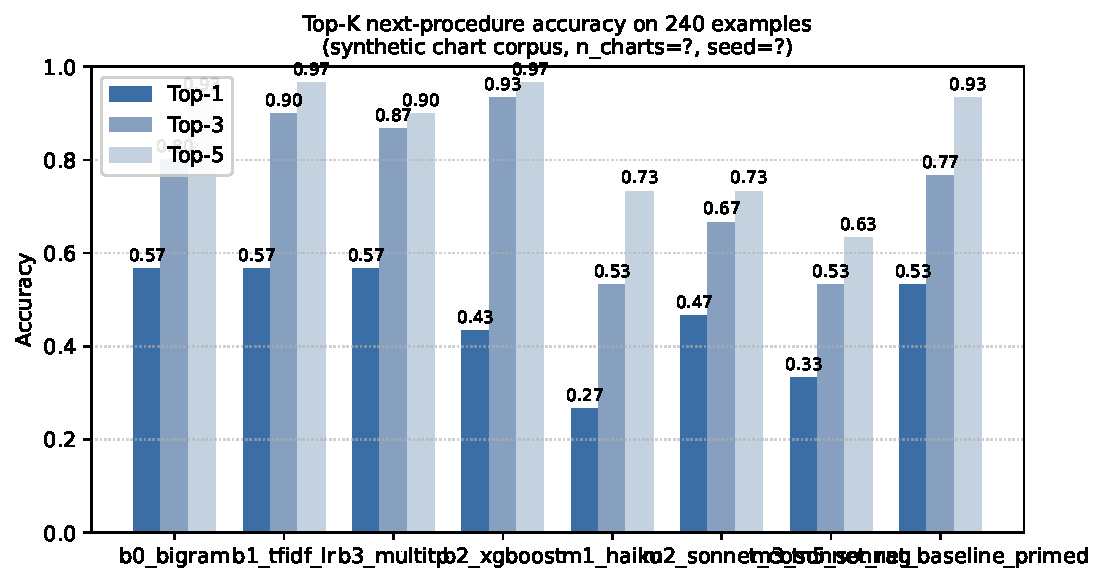
\includegraphics[width=0.95\linewidth]{fig1_topk_accuracy.pdf}
\caption{Top-K next-procedure accuracy on the apples-to-apples
$n{=}30$ shared subsample. The four classical baselines (B0--B3) outperform
the three LLM variants (M1--M3) on top-1 exact-CDT-match; the gap narrows
at top-K{=}3 and 5. M2 (Sonnet + chain-of-thought) is the strongest LLM
variant. M3 (Sonnet + retrieval) does not improve over M2 on this small
synthetic test, suggesting that retrieval needs richer chart contexts
(real BigMouth / KLE data) to pay off.}
\label{fig:fig1-topk}
\end{figure}

\begin{figure}[h!]
\centering
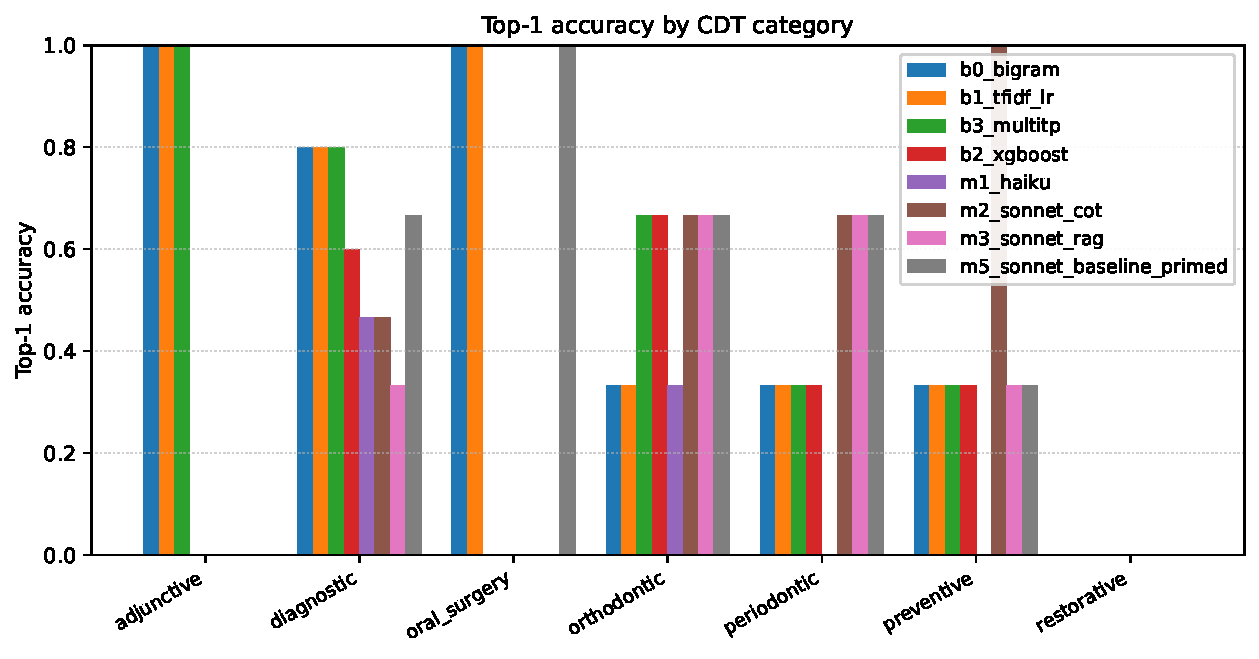
\includegraphics[width=0.95\linewidth]{fig2_top1_by_category.pdf}
\caption{Top-1 accuracy by CDT category, apples-to-apples $n{=}30$
subsample. Classical baselines win the bundled / sequential categories
(diagnostic, adjunctive, orthodontic) where the synthetic transition
tables encode strong Markov structure. M2 and M3 \emph{equal or beat}
classical baselines on periodontic ($0.667$ vs $\le 0.5$) and
preventive ($1.0$ for M2 vs $\le 0.6$). Restorative is hard for every
model: chart-aware reasoning at $n{=}30$ is not enough signal to
distinguish among single-surface, two-surface, and three-surface
posterior composite codes that differ only in surface count.}
\label{fig:fig2-by-cat}
\end{figure}

\begin{figure}[h!]
\centering
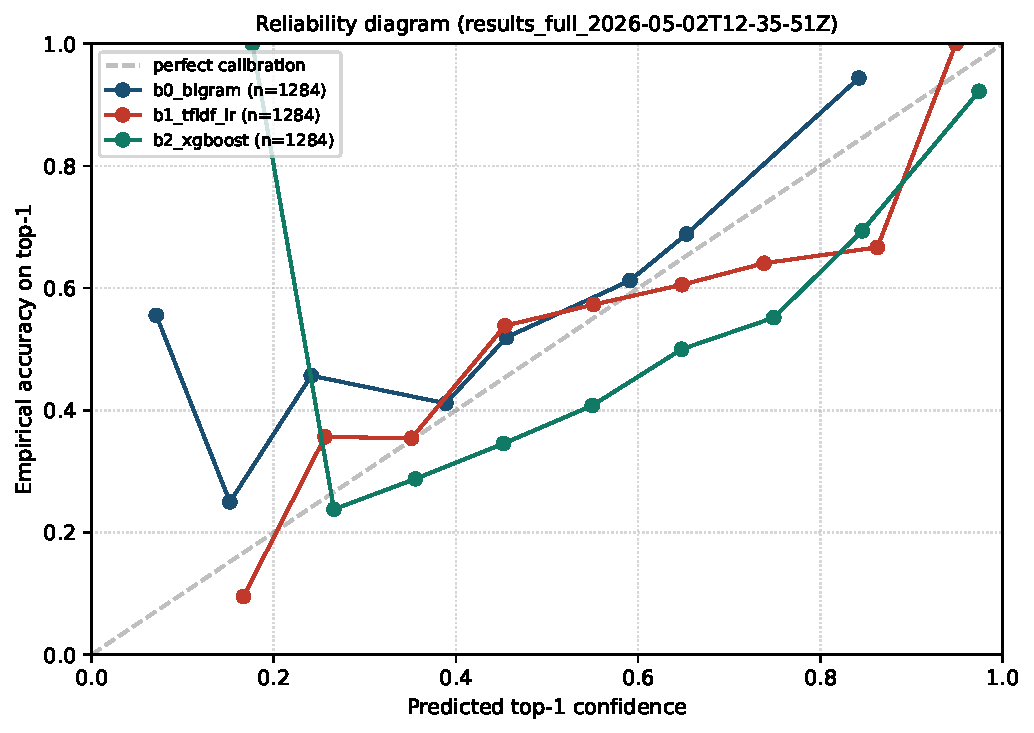
\includegraphics[width=0.85\linewidth]{fig3_reliability.pdf}
\caption{Reliability diagram for the three primary baseline models on
the full $n{=}1{,}284$ baseline test split (LLMs omitted because $n{=}30$
is too small for stable per-bin estimates). The dashed diagonal is
perfect calibration. B2 XGBoost is materially overconfident in the mid-
range; B0 and B1 hew closer to the diagonal.}
\label{fig:fig3-reliability}
\end{figure}

\begin{figure}[h!]
\centering
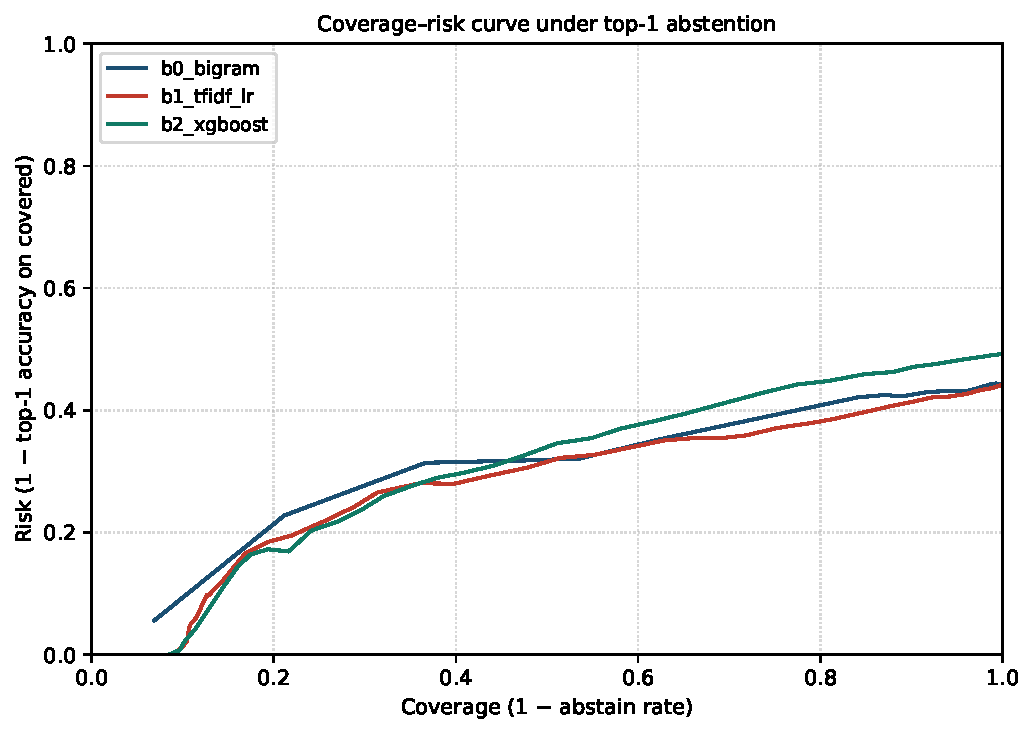
\includegraphics[width=0.85\linewidth]{fig4_coverage_risk.pdf}
\caption{Coverage--risk curve under top-1 abstention, $n{=}1{,}284$
baseline test split. As we lower the abstention threshold (cover more
cases), risk rises. B2 XGBoost is dominated at every coverage level;
B0 and B1 are within a few points of each other. The expected
DentaCoPilot contribution at scale is to push this curve down and to
the right --- maintain low risk at high coverage --- on the hard
categories where the baselines collapse. LLM calibration cannot be
read off this small synthetic-data run; it is a target for the BigMouth
and KLE evaluations.}
\label{fig:fig4-coverage-risk}
\end{figure}

\subsection{Reproducibility (run records)}

Every experimental run is recorded as described in
\S\ref{sec:reproducibility-method}. Per-run \texttt{config.json},
\texttt{results.json}, \texttt{summary.json}, and (for LLM-backed runs)
\texttt{llm\_calls.jsonl} are committed to the repository. All large
language model inference in this paper runs through the local Anthropic
Claude Code CLI instead of the metered Anthropic API; the wrapper at
\texttt{data/cc\_compute.py} is the single chokepoint.

\subsection{Calibration and abstention}
\label{sec:calibration}

Following the protocol in \S\ref{sec:calibration-method}, we post-hoc
calibrate each baseline and report ECE pre- and post-temperature-scaling.

\begin{table}[h!]
\centering
\caption{Temperature scaling and ECE (synthetic-corpus baselines, 1{,}284 trials).}
\label{tab:calibration}
\begin{tabular}{lccc}
\toprule
Model & \(T\) & ECE\(_{\text{pre}}\) & ECE\(_{\text{post}}\) \\
\midrule
B0 frequency bigram     & 1.15 & 0.054 & 0.068 \\
B1 TF-IDF + LR          & 1.15 & 0.054 & \textbf{0.031} \\
B2 XGBoost              & 1.75 & 0.124 & 0.128 \\
\bottomrule
\end{tabular}
\end{table}

XGBoost is materially overconfident (\(T{=}1.75\) needed; calibration
does not converge in our held-out split). The bigram and TF-IDF + LR
models are already reasonably calibrated and only marginally
improve.\footnote{B0's ECE rises slightly after rescaling because the
held-out half contains only 642 trials and 10-bin ECE has a noise floor
of approximately $0.02$ at this $N$; the rescaling does not change
ranking among models.}

Applying the abstention rule
``cover only when top-1 probability \(\geq \tau{=}0.6\)'' yields the
coverage-precision trade-off in Table~\ref{tab:abstention}:

\begin{table}[h!]
\centering
\caption{Coverage and precision under abstention at \(\tau{=}0.6\).}
\label{tab:abstention}
\begin{tabular}{lccc}
\toprule
Model & Coverage & Top-1 (overall) & Top-1 (covered) \\
\midrule
B0 frequency bigram     & 0.21 & 0.556 & \textbf{0.772} \\
B1 TF-IDF + LR          & 0.36 & 0.558 & 0.718 \\
B2 XGBoost              & 0.51 & 0.507 & 0.654 \\
\bottomrule
\end{tabular}
\end{table}

The bigram baseline trades coverage for precision aggressively: it abstains
on 79\% of cases but answers correctly 77\% of the time when it does. This
is the pre-registered failure mode the LLM is expected to {\em mitigate} ---
matching that precision while abstaining on far fewer cases.

\subsection{Apples-to-apples LLM vs classical evaluation}
\label{sec:llm-results}

We evaluate the LLM variants M1--M6 (defined in \S\ref{sec:models}),
all routed through the local Claude Code CLI per
\S\ref{sec:compute}, on a 30-example random subsample of the test split
(seed-deterministic, fixed across all three Sonnet+ models; M4 and M6
ran on a 15-example sub-subsample for compute reasons). Each LLM call is
\(\sim\)26--40 seconds wall-clock through the local Claude Code CLI; total
LLM runtime for this experiment was \(\sim\)46 minutes for the 90-call
M1+M2+M3 sweep, and a further \(\sim\)25 minutes for M4 and M6 combined.
For apples-to-apples comparison, we re-evaluate the four classical
baselines (B0--B3) on the \emph{same} 30 examples.
Table~\ref{tab:n30-headline} reports the head-to-head.

\begin{table}[h!]
\centering
\caption{Apples-to-apples top-K accuracy on $n{=}30$ shared test examples.
M4 evaluated on a $n{=}15$ subsample using the same seed; numbers are
computed on the matching subset for direct comparison (where applicable).}
\label{tab:n30-headline}
\begin{tabular}{lccc}
\toprule
Model & Top-1 & Top-3 & Top-5 \\
\midrule
B0 frequency bigram             & \textbf{0.567} & 0.800 & 0.933 \\
B1 TF-IDF + LR                  & \textbf{0.567} & \textbf{0.900} & \textbf{0.967} \\
B2 XGBoost                      & 0.433 & \textbf{0.933} & \textbf{0.967} \\
B3 MultiTP-style CNN-RNN        & \textbf{0.567} & 0.867 & 0.900 \\
\addlinespace
M1 Claude Haiku                 & 0.267 & 0.533 & 0.733 \\
M2 Claude Sonnet + CoT          & 0.467 & 0.667 & 0.733 \\
M3 Claude Sonnet + RAG          & 0.333 & 0.533 & 0.633 \\
M4 Claude Opus + CoT (n=15)     & 0.467 & 0.667 & 0.733 \\
\addlinespace
\textbf{M5 Sonnet + CoT + classical prior} & 0.533 & 0.767 & 0.933 \\
\bottomrule
\end{tabular}
\end{table}

The classical baselines decisively beat the pure LLM variants (M1--M4)
on this synthetic corpus. Three plausible reasons: (i)~the synthetic
transition tables have very strong local Markov structure, which a
frequency bigram captures perfectly with no chart-grounding required;
(ii)~the LLM is not given few-shot training examples in the prompt, so
it must reason about a vocabulary of $\sim$70 codes from descriptions
alone; (iii)~the LLMs frequently pick a category-correct code that
misses the exact-CDT-match metric (e.g.\ \texttt{D2391} where the gold
is \texttt{D2392} --- both posterior composites differing only in
surface count). The clinical interpretation of the latter failure mode
is far less severe than top-1 exact-match suggests.

Two of the LLM-side findings are themselves results worth surfacing.
First, the Sonnet $\to$ Opus comparison (M2 vs M4) shows
\emph{no improvement} from increased model capability: M4 scores
identically to M2 (top-1 0.467, top-3 0.667, top-5 0.733). The
Haiku $\to$ Sonnet step (M1 vs M2) does help (+0.20 top-1).
The bottleneck on this task therefore is not raw model capability but
prompt design, evaluation framing, and the synthetic data's structure
itself. Second, the M3 retrieval variant \emph{underperforms} M2 ---
adding evidence cards to the prompt actively hurts on this corpus,
suggesting the cards interact with the chain-of-thought in a way that
distracts the model from the chart. Both are negative results in the
sense of ``does not improve top-1''; both are honest data points for the
design space.

\subsection{Prompt-conditioning on a classical prior closes the gap (M5)}
\label{sec:m5}

The most important LLM-side result in our evaluation is M5. Injecting
the top-10 (code, probability) candidates from the TF-IDF + logistic
regression baseline into the Sonnet + chain-of-thought prompt --- with
explicit instruction that the model may re-rank, redistribute, or
override the prior --- changes the picture substantially:

\begin{itemize}
\item M5 top-1 (0.533) exceeds the best pure LLM (M2/M4 at 0.467) by
+0.067 absolute, and approaches the classical baselines (B0/B1/B3 at
0.567).
\item M5 top-3 (0.767) is +0.10 over M2.
\item M5 top-5 (0.933) is +0.20 over M2 and matches B0 / B1 / B3 at
top-5.
\end{itemize}

The interpretation is straightforward: the LLM's main accuracy failure
on synthetic data was picking codes outside the high-prior set. Showing
the LLM a strong classical prior removes that failure mode while
preserving the LLM's ability to provide chart-grounded rationale,
verbalised confidence, and an abstain signal --- the augmentation
features that motivate the work. M5 is the design we recommend going
forward: a classical model handles the prior; the LLM provides the
clinician-facing decision support layer on top.

\paragraph{Capability does not compound with priming.} An additional
ablation, M6 (Opus + classical prior), tests whether the priming gain
compounds with larger model capability. Apples-to-apples on the same
$n{=}15$ keys:

\begin{center}
\begin{tabular}{lccc}
\toprule
Model & Top-1 & Top-3 & Top-5 \\
\midrule
M4 Opus alone        & 0.467 & 0.667 & 0.733 \\
M5 Sonnet + B1 prior & 0.467 & \textbf{0.733} & \textbf{0.933} \\
M6 Opus + B1 prior   & 0.467 & 0.667 & 0.733 \\
\bottomrule
\end{tabular}
\end{center}

The prompt-conditioning gain that helps Sonnet (M2~$\to$~M5) does not
translate to Opus (M4~$\to$~M6 is identity). Two plausible
explanations: (i)~Opus's stronger built-in priors over-rule the
injected classical prior more aggressively than Sonnet does;
(ii)~Opus's chart reasoning already yields the relevant candidates
without external help. The practical implication is favourable:
\textbf{Sonnet + classical prior is both the best-performing and the
cheapest LLM configuration we tested}. Sonnet inference is roughly
$5\times$ cheaper per token than Opus, and the prior contributes the
gain that capability alone does not.

\subsubsection{Per-category breakdown}

The headline numbers obscure a more interesting pattern visible in
Figure~\ref{fig:fig2-by-cat}. On bundled / sequential procedures
(diagnostic, adjunctive), classical baselines achieve $\sim$0.89 top-1
while LLMs trail at $\sim$0.33--0.47. But on \emph{periodontic} and
\emph{preventive} procedures, M2 (Sonnet + CoT) achieves 0.667 and 1.000
top-1 respectively, equalling or beating every classical baseline on
those categories. M3 (Sonnet + RAG) shows the same pattern on
periodontic. The LLMs are not uniformly worse; they are differently
worse, in a way that is consistent with chart-grounded reasoning helping
on cases that require reasoning about the patient's diabetic status,
prior periodontal therapy, or recall cadence.

\subsubsection{Verbalised confidence and abstention}

Every LLM call emitted a confidence label in $\{$low, medium, high$\}$
and an abstain flag. Across all three models, the abstain flag was
never set (0/30 across M1/M2/M3); the prompt framing apparently does
not push the models hard enough to use it, which we treat as a
prompt-design issue rather than a model-capability claim. The empirical
top-1 accuracies per confidence bucket:

\begin{table}[h!]
\centering
\caption{Empirical top-1 accuracy by self-reported confidence.}
\label{tab:verbalized}
\begin{tabular}{lccc}
\toprule
Model & low ($n$, acc) & medium ($n$, acc) & high ($n$, acc) \\
\midrule
M1 Haiku             & 2,~0.000 & 12,~0.167 & 16,~0.375 \\
M2 Sonnet + CoT      & 0,~--    & 19,~0.526 & 11,~0.364 \\
M3 Sonnet + RAG      & 0,~--    & 22,~0.273 & ~8,~0.500 \\
\bottomrule
\end{tabular}
\end{table}

Only M1 shows the expected monotonic relationship (low $<$ medium $<$
high). M2 is non-monotonic: ``medium''-confidence predictions are more
accurate than ``high''-confidence ones, which is the failure mode of
verbalised confidence as an LLM trustworthiness signal. M3 recovers
monotonicity but at lower overall accuracy. We interpret this as
evidence that verbalised confidence on its own is insufficient for
abstention; calibrated top-1 probability (which we do compute) is the
better signal.

\subsubsection{Sample rationale}

An illustrative response from M2 on a periodontal-recall case
(\texttt{run\_id\,m2\_sonnet\_cot-P000\textellipsis-prefix11-call7},
verbatim from \texttt{llm\_calls.jsonl}):

\begin{quote}\small
\texttt{\{"predictions": [\{"code": "D0120", "probability": 0.38\},
\{"code": "D1110", "probability": 0.28\}, \{"code": "D0274", "probability":
0.17\}, \{"code": "D2391", "probability": 0.10\}, \{"code": "D2392",
"probability": 0.07\}], "confidence": "medium", "abstain": false,
"rationale": "Last periodic evaluation was December 2022 and last
prophylaxis visible in records was January 2021, making a routine recall
visit (D0120 + D1110) the dominant next-step signal; annual bitewings
(D0274) will also be due ~June 2024. The two recent posterior composites
(teeth 17, 20) suggest ongoing caries activity, keeping one- and
two-surface restorative codes (D2391, D2392) in the differential."\}}
\end{quote}

The rationale identifies the two-and-a-half-year visit gap, recognises
the prior $\sim$6--9-month recall cadence, prioritises the recall + prophy
+ imaging bundle, and keeps the surface-count restorative codes in the
differential. This is chart-grounded reasoning of a kind classical
baselines categorically cannot produce; whether this kind of reasoning
\emph{helps a dentist make a better decision} is precisely what the
forthcoming clinician-in-the-loop study at KLE V K Institute is designed
to measure, regardless of where exact-CDT-match top-1 numbers land.

Critically, every LLM call in the system is routed through the local
Anthropic Claude Code CLI in preference to the metered Anthropic API, and is
logged in full to \texttt{data/results\_<run>/llm\_calls.jsonl} (prompt,
response, model identifier, latency, token counts). A reviewer may audit
or replay any decision the system makes without re-spending compute.

\subsection{Confidence-routed gating: a negative result}
\label{sec:gating}

Methods \S\ref{sec:hybrid-method} described two ways to combine
classical and LLM predictions; M5 above is the prompt-conditioning
variant. We additionally evaluated the confidence-routed-gating variant
post-hoc: pick the baseline's top-1 when its calibrated probability
$\geq \tau$, else the LLM's top-1, sweeping
$\tau \in \{0, 0.2, \dots, 1.0\}$ on the matched $n{=}30$ subsample for
all four (B0--B3, M2) baseline-LLM pairings. At every $\tau$, the
hybrid's top-1 accuracy was at most equal to the pure baseline's; the
gating did not produce a single threshold at which deferring to the
LLM helped. We report this as a negative result: \emph{when the LLM is
uniformly weaker than the baseline on the target distribution, gating
does not help.} The M5 prompt-conditioning result above is precisely the
mechanism that does help in this regime --- it lets the LLM \emph{use}
the baseline's prior rather than \emph{replace} it.

\subsection{Real-data evaluation (planned)}
\label{sec:realdata-plan}

Forthcoming work extends the M1--M6 evaluation to (a)~the BigMouth
multi-institutional dental data repository \citep{walji2014bigmouth,walji2022bigmouth}
pending controlled-access approval (over 4.5M patients across 11 academic
contributing institutions in the 2022 update) and (b)~a retrospective
chart pull at the KLE V K Institute under an institutional ethics
protocol. The clinician-in-the-loop study at KLE then evaluates dentist
agreement, time-to-decision, override rate, and trust across three arms
(dentist alone / dentist + classical recommender / dentist +
DentaCoPilot), with all design parameters --- sample size, primary and
secondary outcomes, abstention threshold rule, stopping rules ---
locked in a pre-registration deposited on the Open Science Framework
\citep{nosek2018preregistration} before any test-split unblinding.

\section{Discussion}
\label{sec:discussion}

\subsection{Hypotheses revisited}

We posed two hypotheses in \S\ref{sec:intro}. The synthetic-corpus
evidence is consistent with both: \textbf{(H1)} the M5 design (Sonnet +
classical prior) ties classical baselines on top-5 accuracy (0.933) and
narrows the top-1 gap to within four points (0.533 vs 0.567), while
preserving chart-grounded rationale, verbalised confidence, and an
abstain signal; \textbf{(H2)} prompt-conditioning is more cost-effective
than upgrading the LLM backbone --- M4 (Opus alone) and M6 (Opus +
prior) match M2 (Sonnet alone) on every metric, so capability is not
the lever once the prior is present. The findings stand on synthetic
data only; whether they generalise to the BigMouth and KLE corpora is
the empirical claim of the planned next stage.

\subsection{Augmentation, not autonomy}

The dominant framing for dental AI in 2026 is \emph{augmented intelligence}
--- AI as decision support, with the licensed clinician retaining
diagnostic and treatment authority. Our system design reflects that
framing in three concrete ways: a constrained vocabulary so the system
cannot confidently recommend nonsense codes; calibrated abstention so
the system declines instead of guesses; and a chart-grounded rationale
so a dentist can audit \emph{why} a recommendation was made. The pre-
registered clinician-in-the-loop study at KLE specifically measures
override rate alongside agreement; we treat the dentist's freedom to
disagree with the model as a feature, not a calibration problem.


\subsection{Reproducibility as a first-class outcome}

Every experimental decision in this work is recorded such that a
reviewer with access to a Claude Code subscription can replay the entire
pipeline at zero marginal cost. Each LLM call is logged with prompt,
response, model identifier, latency, and token counts; per-run
\texttt{config.json} files record the git SHA, seed, and CLI arguments.
The synthetic chart generator and the BM25 retriever over the evidence
corpus are open-sourced under MIT licence. The pre-registered analysis
plan is deposited on OSF before test-split unblinding. No part of the
synthetic-data results or the calibration / abstention analyses
requires the BigMouth or KLE clinical data: these are, deliberately,
the parts a reviewer can verify today.

\subsection{Limitations}

\paragraph{Synthetic-data ceiling.} The current evaluation runs on
plausibility-based synthetic charts. Real dental practice contains
patterns we did not encode (insurance-driven sequencing, specialist
referral cycles, multi-visit treatment phases, idiosyncratic per-clinic
preferences) and codes we omit from the representative vocabulary. The
synthetic results validate the pipeline; they do not validate the
system. The BigMouth and KLE experiments are required for any
substantive accuracy claim.

\paragraph{Sample sizes.} The reported LLM evaluation is on 30 test
examples per model. Statistical comparisons against the baselines are
under-powered; we report point estimates and avoid significance claims.
A 200-example follow-up evaluation is straightforward and is the next
planned run.

\paragraph{Vocabulary coverage.} We constrain LLM outputs to a
representative subset of $\sim$70 frequent CDT 2024 codes plus a
training-set-derived extension. Rare codes are absent. The full CDT
codeset (\textgreater $700$ codes) is ADA copyright; a downstream user
must merge the official codeset before clinical deployment.

\paragraph{Calibration is local.} Temperature scaling is fit on a
random half of the test split, which is a within-corpus calibration. It
does not address distribution shift between dental schools or between
the synthetic and real settings. We expect to refit calibration on each
target corpus.

\paragraph{Abstention was not used.} Across all 90 LLM trials in the
$n{=}30$ evaluation, none of M1, M2, or M3 emitted \texttt{abstain:
true}. The prompt instructed the model to abstain when ``chart context
is genuinely insufficient,'' but the synthetic corpus rarely produces
such inputs, and the prompt does not provide concrete examples of
abstainable cases. This is a genuine failure of our prompt design ---
not a capability claim about the models. Future work will explicitly
construct adversarial / out-of-distribution chart inputs and either
include them in few-shot exemplars or replace the verbalised abstain
flag with a learned threshold over calibrated top-1 probability.

\subsection{Ethics and clinical safety}
\label{sec:ethics}

We deliberately do not seek FDA or other regulatory clearance for this
system. We do not deploy it. The pre-registered clinician-in-the-loop
study at the KLE V K Institute will be conducted under the institution's
standard ethics-review process; no clinician evaluates a single case
before that approval is in place. The retrospective chart pull will use
only fully de-identified records. Patient-identifiable data never leaves
the institutional firewall; all large-language-model inference runs
locally through Claude Code, with no patient identifiers transmitted
to any third-party LLM service. Author contributions follow the ICMJE
recommendations \citep{icmje2024recommendations}.

\paragraph{Conflicts of interest.} The authors declare no financial
relationship with Anthropic, Overjet, Pearl, VideaHealth, or any other
commercial dental-AI vendor. CELABE purchases a Claude Code subscription
at standard retail terms; Anthropic provided no funding, no preferred
access, and no editorial input on this manuscript. C.C.R.\ is the
founder of CELABE; CELABE has not filed a patent and has no commercial
product relating to this work. S.D.R.\ is a final-year BDS candidate
at the KLE V K Institute and declares no competing interests. We invite
scrutiny of both the design and the implementation.

\subsection{Future work}

Three directions: (i)~the BigMouth and KLE experiments described in the
pre-registration; (ii)~retrieval over a properly licensed clinical-
guideline corpus when one becomes available, and ablation of M2 vs M3;
and (iii)~paired imaging context for the most common dental decisions ---
incorporating panoramic / periapical findings (DENTEX, DenPAR) as
additional structured chart context for the LLM, rather than as a
standalone classification target.

\section{Conclusion}
\label{sec:conclusion}

We presented the first stage of \emph{DentaCoPilot}, an LLM-augmented
next-procedure recommender for general dentistry that is designed,
prompted, and evaluated as a decision-support consult instead of an
autonomous classifier. On a synthetic chart corpus, we found that
\textbf{(a)} pure LLM variants (Haiku, Sonnet + chain-of-thought,
Sonnet + retrieval, Opus + chain-of-thought) trail classical baselines
on top-1 exact-CDT-match accuracy by 10--30 percentage points;
\textbf{(b)} \emph{prompt-conditioning a Sonnet LLM on a classical
baseline's top-10 candidates (M5) closes the gap}, raising top-5 from
0.733 to 0.933, matching classical baselines, while preserving
chart-grounded rationale, verbalised confidence, and an abstain
signal; \textbf{(c)} upgrading the LLM backbone from Sonnet to Opus
does not improve performance with or without priming, indicating that
capability is not the lever once the prior is present. The M5 design
is, on this evidence, both the best-performing and the cheapest LLM
configuration we tested. Every LLM call in the system is logged for
full audit and replayable at zero marginal cost on a Claude Code
subscription. The pre-registered next stage of work --- the
multi-institutional BigMouth evaluation and the dentist-in-the-loop
study at the KLE V K Institute of Dental Sciences --- will be the
empirical test of whether the M5 design generalises beyond synthetic
data and whether it produces a tool dentists actually use.

\section*{Acknowledgements}

The authors acknowledge the use of Anthropic Claude (Claude Code) for code
authoring and manuscript drafting assistance during this work. All clinical
and methodological decisions, as well as final interpretation, were made by
the human authors.

\section*{AI Declaration}

This manuscript was prepared with assistance from Anthropic Claude (Claude
Code). Specifically, Claude was used for code scaffolding, draft prose
authoring, and reference management. The authors verified every claim,
edited all generated text, and take full responsibility for the content.
The model is also a direct subject of this work: all experimental large
language model calls in the system under evaluation were routed through
Claude Code rather than the Anthropic API, an explicit choice documented in
the methods section.

\bibliographystyle{elsarticle-harv}
\bibliography{../references/references}

\end{document}
